\section{Classification}

\subsection{ML System Classification}
There are three types of machine learning systems:

\begin{description}
	\item [\cindex{supervised learning}] training data comes with solution called \cindex{labels}. It has two kinds of tasks:
		\begin{description}
			\item [\cindex{classification}] target is discrete value
			\item [\cindex{regression}] target is continuous value
		\end{description}
	\item [\cindex{unsupervised learning}] the training data is unlabeled. It has these tasks:
		\begin{itemize}
			\item clustering
			\item visualization 
			\item dimension reduction
			\item anomaly detection
		\end{itemize}
	\item [\cindex{semi-supervised learning}] it has a lot of unlabeled data and a little labeled data. One example is to group photo by person, which is unsupervised, then by labelling one person all data could be labeled
	\item [\cindex{reinforcement learning}] build on Markov Decision Process
\end{description}

\subsection{Batch and Online Learning}

In \cindex{batch learning} the system is trained and then launched into production without any learning. The training might take hours to finish.

In \cindex{online learning}, the system is feed with data sequentially, either individually or in small \cindex{mini-batches}. The training is fast and the data could be discarded after learning.

In \cindex{out-of-core} learning, online learning algorithm is used to train system on huge data set that cannot fit into memory.

\subsection{learning rate}

In \cindex{online learning} the \cindex{learning rate} needs to be carefully controlled. If it is set to too high, the system will rapidly adapt to new data, or noisy data. The system need to closely monitor the performance and turn off \cindex{online learning} on performance degradation. 

\begin{itemize}
	\item high: short term memory and can learn quickly
	\item low: less sensitive to noisy data but learn slowly
\end{itemize}


\subsection{Test and Validation}

The data is splitted into three sets:
\begin{itemize}
	\item training set
	\item validation set
	\item test set
\end{itemize}

The training process is:
\begin{itemize}
	\item run model on \cindex{training set}
	\item select the best one based on \cindex{validation set} 
	\item generate model error based on \cindex{test set}
\end{itemize}


\subsection{Feature Engineering}

\cindex{feature engineering}:
\begin{itemize}
	\item feature selection
	\item feature extraction
\end{itemize}

\subsection{Data Cleaning}

There are few useful data cleaning methods:
\begin{itemize}
	\item scaling
		\begin{itemize}
			\item min-max scaling: scale to $[0,1]$
			\item standardization: scale to zero mean and unit variance.
		\end{itemize}
	\item string handling
		\begin{itemize}
			\item encode label: convert string to enumeration
			\item one-hot encoder: convert string to a $0$-$1$ matrix
			\item label binarizer: enable label and one-hot encoder together
		\end{itemize}
	\item NAN handling: replace NAN by median
	\item polynomial change: change number using polynomial function
\end{itemize}

\subsection{regularization}

use \cindex{hyperparameter} to control the risk of overfitting.


\subsection{Tune Model}
two different model tuning methods:
\begin{itemize}
	\item grid search: generate a combination of parameters and search
	\item randomized search
\end{itemize}



\subsection{Cross Validation}

Split the training data into $k$ groups. Train the data on $k-1$ group and use the remaining one for validation.

Still need to use a separate test set.


\subsection{Precision, Recall, ROC}

\begin{equation}
	\text{precision} = \frac{TP}{TP + FP}
\end{equation}

\begin{equation}
	\text{recall} = \frac{TP}{TP + FN}
\end{equation}

\begin{equation}
	\text{false positive rate} = \frac{FP}{FP + TN}
\end{equation}

There is a trade-off between \cindex{precision} and \cindex{recall}. Given a fixed model and prediction, when the threshold increases, the \cindex{precision} might increase (it could decrease) and the \cindex{recall} will always decrease. 

\cindex{confusion matrix} (\cindex{PR curve}) is a plot between \cindex{precision} and \cindex{recall}. 

\begin{figure}[H]
\centering	
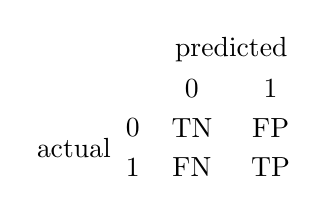
\begin{tikzpicture}
	\node at (1,3) {predicted};
	\node at (0.5,2.5) {$0$};
	\node at (1.5,2.5) {$1$};
	\node at (0.5,2) {TN};
	\node at (1.5,2) {FP};
	\node at (0.5,1.5) {FN};
	\node at (1.5,1.5) {TP};
	\node at (-0.25,2) {$0$};
	\node at (-0.25,1.5) {$1$};
	\node at (-1,1.75) {actual};
\end{tikzpicture}

\caption{confusion matrix}
\end{figure}


\cindex{receiver operating characteristic} (ROC) is a plot between \cindex{recall} and $1 - \text{specificity}$.

\cindex{PR curve} is preferred when:
\begin{itemize}
	\item positive rate is rare
	\item care more about false positive than false negative
\end{itemize}

\begin{figure}[H]
\centering	
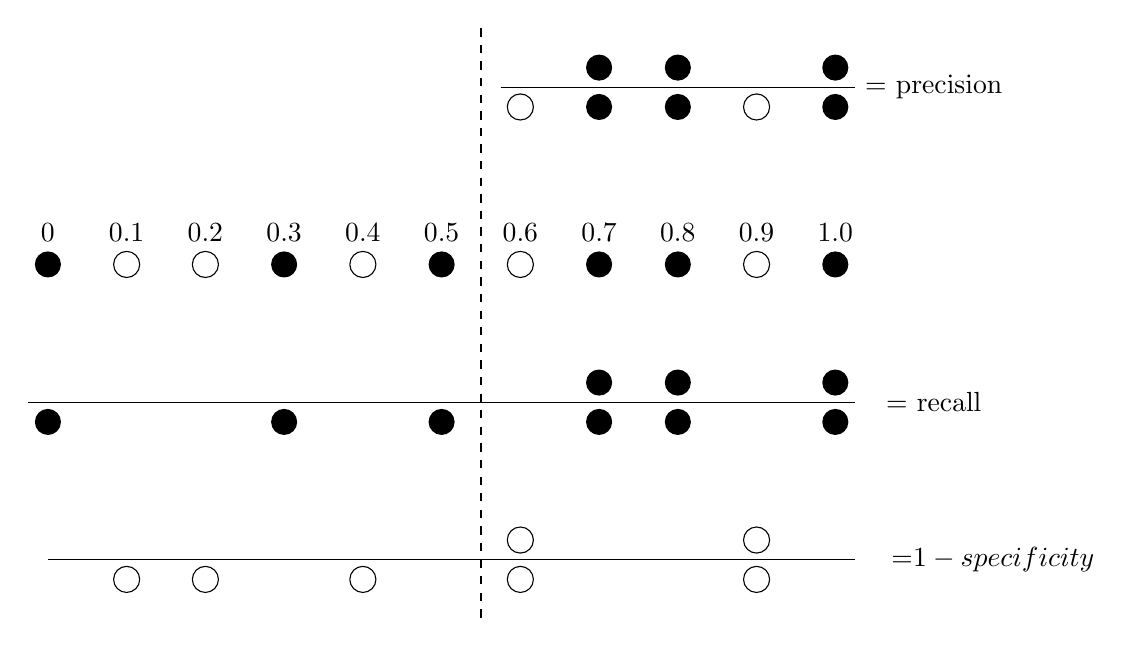
\begin{tikzpicture}
	\node [circle,fill] (s) [label=$0$] at (0,0) {};
	\node [circle,draw] (s) [label=$0.1$] at (1,0) {};
	\node [circle,draw] (s) [label=$0.2$] at (2,0) {};
	\node [circle,fill] (s) [label=$0.3$] at (3,0) {};
	\node [circle,draw] (s) [label=$0.4$] at (4,0) {};
	\node [circle,fill] (s) [label=$0.5$] at (5,0) {};
	\node [circle,draw] (s) [label=$0.6$] at (6,0) {};
	\node [circle,fill] (s) [label=$0.7$] at (7,0) {};
	\node [circle,fill] (s) [label=$0.8$] at (8,0) {};
	\node [circle,draw] (s) [label=$0.9$] at (9,0) {};
	\node [circle,fill] (s) [label=$1.0$] at (10,0) {};
	
	% draw the threshold
	\draw [dashed] (5.5,3) -- (5.5,-4.5);
	
	% draw precision
	\node [circle,draw] (s) at (6,2) {};
	\node [circle,fill] (s) at (7,2) {};
	\node [circle,fill] (s) at (8,2) {};
	\node [circle,draw] (s) at (9,2) {};
	\node [circle,fill] (s) at (10,2) {};
	
	\draw (5.75,2.25) -- (10.25,2.25);

	\node [circle,fill] (s) at (7,2.5) {};
	\node [circle,fill] (s) at (8,2.5) {};
	\node [circle,fill] (s) at (10,2.5) {};
	
	\node at (11.25,2.25) {= precision};
	
	% draw recall
	\node [circle,fill] (s) at (0,-2) {};
	\node [circle,fill] (s) at (3,-2) {};
	\node [circle,fill] (s) at (5,-2) {};
	\node [circle,fill] (s) at (7,-2) {};
	\node [circle,fill] (s) at (8,-2) {};
	\node [circle,fill] (s) at (10,-2) {};
	
	\draw (-0.25,-1.75) -- (10.25,-1.75);
	
	\node [circle,fill] (s) at (7,-1.5) {};
	\node [circle,fill] (s) at (8,-1.5) {};
	\node [circle,fill] (s) at (10,-1.5) {};
	
	\node at (11.25,-1.75) {= recall};
	
	% ROC
	
	\node [circle,draw] (s) at (1,-4) {};
	\node [circle,draw] (s) at (2,-4) {};
	\node [circle,draw] (s) at (4,-4) {};
	\node [circle,draw] (s) at (6,-4) {};
	\node [circle,draw] (s) at (9,-4) {};
	
	\draw (0,-3.75) -- (10.25,-3.75);
	
	\node [circle,draw] (s) at (6,-3.5) {};
	\node [circle,draw] (s) at (9,-3.5) {};
	
	\node at (12,-3.75) {=$1 - \text{specificity}$};
\end{tikzpicture}
\caption{PR and ROC curve}
\end{figure}

\subsection{Prediction Output Format}

\begin{description}
	\item [binary] the output is binary: $O \in \{ 0, 1\}$. such as \cindex{SVM}. 
	\item [multiclass] output can be of $n$ value: $O \in \{ 0,1,2,3\}$
		\begin{itemize}
			\item OvA: binary classifier that use one feature against all the rest feature. $n$ internal classifiers. select the one with highest score.
			\item OvO: for every feature pair, run a binary classifier. $\binom{n}{2}$ internal classifiers. select the one with highest sum of scores.
			\begin{itemize}
				\item training set needs to be small
				\item usually for \cindex{SVM}
			\end{itemize}
		\end{itemize}
	\item [multilabel] $n$ binary prediction: $[0,1,0,1]$, which means female=false, alice=true, etc. such as k-nearest neighbor. 
	\item [multioutput] $n$ non-binary output: $[1,2,89]$.
\end{description}


\subsection{Optimization}

\subsubsection{Batch Gradient Descent}

\cindex{Gradient descent} is used to minimize cost function. \cindex{Linear regression model} is \cindex{convex}, so it will be guaranteed to find global minimum.

all features need to have a similar scale in order to increase converge speed.

In GD learning, $\eta$ is the learning rate, $\theta$ is model's parameter vector, $f$ (such as MSE) is the cost function. Formula (\ref{gdlearning}) will try to minimize cost function recursively until $|\nabla_\theta f| < \varepsilon$ ($\varepsilon$ is called \cindex{tolerance})

\begin{equation}\label{gdlearning}
	\theta \gets \theta - \eta \nabla_\theta f
\end{equation}

Each iteration will use all input because the cost function is the sum of error over all inputs. So it is called \cindex{batch} and slow on very large data set.

\subsubsection{Stochastic Gradient Descent}

In each iteration just take a random instance in training set. The cost function will fluctuate. 

The SGD has the chance of finding global minimum. The \cindex{learning rate} needs to be reduced gradually in order to let the training converge, which is called \cindex{simulated annealing} process with \cindex{learning schedule}.

\subsubsection{Mini-batch Gradient Decent}

Mini-batch gradient descent the middle between SGD and GD. Each iteration will take a small random set of instance from training set.


\subsection{Learning Curve}

\cindex{Learning curve} is a plot of error against training set size for training set and validation set. 

At the beginning the error for training set is low and gradually increases, and for validation set it is high and gradually decreases. the gap between two sets could be decomposed into 3 components:
\begin{description}
	\item [bias] the model is wrong. usually \cindex{underfit}.
	\item [variance] has excessive parameter. usually \cindex{overfit}
	\item [irreducible error] data is noisy. need to clean data.
\end{description}


\subsection{Regularization}

\subsubsection{Ridge Regression}

also called \cindex{Tikhonov regularization} or $l2$ . It add the following to the cost function:
\begin{equation}
	\alpha \sum_{i=1}^n \theta_i^2
\end{equation}

The extra cost is only added during training and removed in evaluation.

The data set need to be scaled before applying \cindex{ridge regression}.

\subsubsection{Lasso Regression}
\cindex{Lasso regression} (Least absolute shrinkage and selection operator regression) will add the following to the cost function:
\begin{equation}
	\alpha \sum_{i=1}^n |\theta_i|
\end{equation}

unimportant features will have $0$ weight, so it will output a \cindex{sparse model}.

\subsubsection{Elastic Net}
\cindex{Elastic net} is the middle between \cindex{ridge regression} and \cindex{Lasso regression}. It will add the following to cost function:

\begin{equation}
	\frac{1-r}{2} \alpha \sum_{i=1}^n \theta_i^2 + r \alpha \sum_{i=1}^n |\theta_i|
\end{equation}


\subsubsection{Early Stopping}

It stops training when the validation error reaches minimum. 

For mini-batch and stochastic GD, the validation error curve will fluctuate. One solution is to continue run for a while and roll back to previous minimum.


\subsection{Logistic Regression}

\cindex{logistic regression} is a binary classifier. The probability is:

\begin{equation}
	\hat{p} = \frac{1}{1+e^{-\mathbb{\theta}^T  \mathbf{X}}}
\end{equation}

The prediction is:
\begin{equation}
	\hat{y} = \begin{cases}
		0 \text{, if } \hat{p} < 0.5 \\
		1 \text{, if } \hat{p} \geq 0.5
	\end{cases}
\end{equation}

The cost function is:
\begin{equation}
	J(\theta) = - \frac{1}{m} \sum_{i=1}^m \Big\{ y^{(i)} \log \hat{p}^{(i)} + (1-y^{(i)}) \log (1-\hat{p}^{(i)}) \Big\}
\end{equation}

The derivative is:
\begin{equation}
	\frac{\partial J(\theta)}{\partial \theta_j} = \frac{1}{m} \sum_{i=1}^m \Big( \frac{1}{1+e^{-\mathbb{\theta}^T \mathbf{X}^{(i)}}} - y^{(i)} \Big) x_j^{(i)}
\end{equation}


\subsection{Softmax Regression}
\cindex{Softmax regression} is a multiclass version of \cindex{logistic regression} which is defined as:

\begin{equation}
	\hat{p}_k = \frac{e^{\theta_k^T \mathbb{X}}}{\sum\limits_{j=1}^{\mathbf{K}} e^{\theta_j^T \mathbf{X}}}
\end{equation}

Here $\mathbb{K}$ is the number of classes.


The prediction is:
\begin{equation}
	\hat{y} = \underset{k}{\text{argmax }} \theta_k^T \mathbf{X}
\end{equation}

The cost function is:
\begin{equation}
	J(\theta)= -\frac{1}{m} \sum_{i=1}^m \sum_{k=1}^K y_k^{(i)} \log \hat{p}_k^{(i)}
\end{equation}


The gradient vector is:
\begin{equation}
	\nabla_{\theta_k} J(\theta) = \frac{1}{m} \sum_{i=1}^m(\hat{p}_k^{(i)} - y_k^{(i)}) \mathbf{X}^i
\end{equation}